\documentclass[11pt]{beamer}
\setbeamertemplate{bibliography item}{\insertbiblabel}
\usetheme{Singapore}
\usepackage[utf8]{inputenc}
\usepackage{verbatim}
\usepackage{amsmath}
\usepackage{amsfonts}
\usepackage{amssymb}
\usepackage{graphicx}
\usepackage{cancel}
\usepackage{verbatim}
\usepackage[backend=bibtex]{biblatex}
\addbibresource{mybib.bib}
%\setbeamertemplate{bibliography item}{\insertbiblabel}
\author{Bithiah Yuan}
\title{A Comparison of Facial Feature Extraction Methods based on Professional Domain Clustering}
%\setbeamercovered{transparent} 
%\setbeamertemplate{navigation symbols}{} 
%\logo{} 
\date{} 
\institute{\normalsize Master Project \\ University of Freiburg - Department of Compute Science \\ Chair of Databases and Information Systems} 
\setbeamertemplate{footline}[frame number]
 

\begin{document}

\begin{frame}
\titlepage
\end{frame}

\section{Introduction}

\begin{frame}{Introduction}
\begin{tabular}{l}
\parbox{1\linewidth}{
\frametitle{Motivation}
\begin{itemize}
\setlength\itemsep{1em}
\item \textbf{Question:} Can facial features predict a person's professional talents?
\item \textbf{Problem:} Research in the social sciences are limited in scalability, consistency, and generalization
\item \textbf{Solution:} Computational method based on data and face clustering
\end{itemize} }
\end{tabular}    
\end{frame}

\begin{frame}{Face Clustering}
\begin{tabular}{l}
\parbox{1\linewidth}{
\frametitle{Face Clustering}
\begin{itemize}
\setlength\itemsep{1em}
\item Clustering groups data points into clusters based on their similarities \item Group similar faces together and evaluate the clusters
\item The accuracy can determine if facial features are correlated with one's professional domain
\item Face clustering is usually composed of 4 steps
\end{itemize}
}
\end{tabular}  
\end{frame}

\section{Face Clustering}
\begin{frame}{Face Clustering}
\begin{tabular}{l}
\parbox{1\linewidth}{
\frametitle{Face Clustering}
\bigskip
\textbf{1. Face Detection:} Detect the position of the faces in an image and returns the coordinates of a bounding box for each face\\

\textbf{2. Face Alignment:} Find a set of facial landmarks, resize and crop the image to the edges of the landmarks
\begin{figure}[!tbp]
  \centering
  \begin{minipage}[b]{0.49\textwidth}
    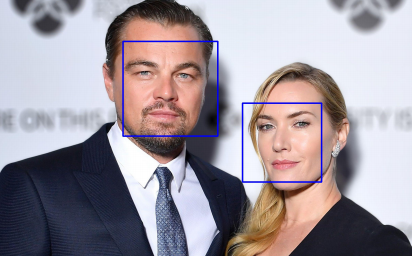
\includegraphics[width=\textwidth]{figures/face_detection.png}
    \caption{Face Detection \cite{trigueros}}
    \label{fig:detect}
  \end{minipage}
    \begin{minipage}[b]{0.49\textwidth}
    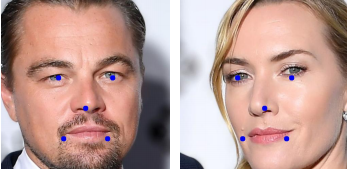
\includegraphics[width=\textwidth]{figures/landmark.png}
    \caption{Face Alignment \cite{trigueros}}
    \label{fig:landmark}
  \end{minipage}
\end{figure}
}
\end{tabular}  
\end{frame}

\begin{frame}{Face Clustering}
\begin{tabular}{l}
\parbox{1\linewidth}{
\frametitle{Face Clustering}
\bigskip
\textbf{3. Face Representation:} Transform the pixel values of a face image into a low-dimensional discriminative feature vector, also known as an \textbf{embedding} \\
\textbf{4. Face Clustering:} Apply clustering algorithm
\begin{figure}[!tbp]
  \centering
  \begin{minipage}[b]{0.4\textwidth}
    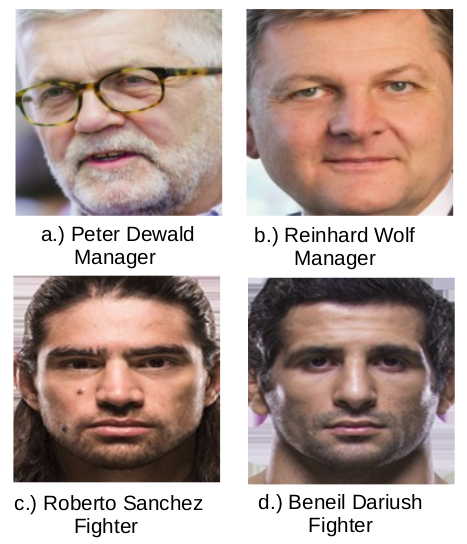
\includegraphics[width=\textwidth]{figures/plot2.png}
  \end{minipage}
\end{figure}
}
\end{tabular}  
\end{frame}

\begin{frame}{Face Clustering}
\begin{tabular}{l}
\parbox{1\linewidth}{
\frametitle{Face Clustering}
\begin{figure}[!tbp]
  \centering
  \begin{minipage}[b]{0.8\textwidth}
    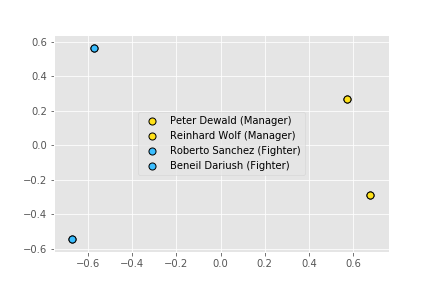
\includegraphics[width=\textwidth]{figures/plot.png}
    \caption{Professional Domain Clustering \cite{trigueros}}
    \label{fig:landmark}
  \end{minipage}
\end{figure}
}
\end{tabular}  
\end{frame}

\section{Face Detection}
\begin{frame}{Face Detection}
\begin{tabular}{l}
\parbox{1\linewidth}{
\frametitle{Histograms of Oriented Gradients (HOG)}
\begin{itemize}
\item HOG divides the image into small grids
\item Each grid accumulates a histogram of gradient directions over the pixels of the grid
\item Trained to classify the region of the face in an image
\item The part of the image that looks most similar to a trained HOG detector will be detected 
\end{itemize}

\begin{figure}[!tbp]
  \centering
  \begin{minipage}[b]{0.25\textwidth}
    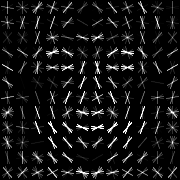
\includegraphics[width=\textwidth]{figures/hog_dlib.png}
    \caption{Trained HOG detector \cite{trigueros}}
    \label{fig:dlibhog}
  \end{minipage}
  \hfill
  \begin{minipage}[b]{0.45\textwidth}
    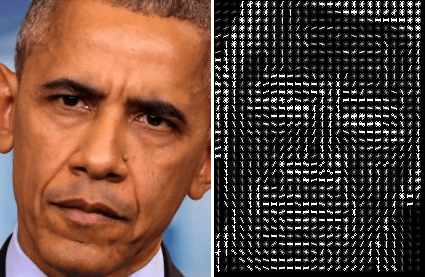
\includegraphics[width=\textwidth]{figures/face_hog.png}
    \caption{HOG representation \cite{hackevolve}}
    \label{fig:obama}
  \end{minipage}
\end{figure}
}
\end{tabular}  
\end{frame}

\iffalse
\begin{frame}{Face Detection}
\begin{tabular}{l}
\parbox{1\linewidth}{
\frametitle{Landmark Detector}
\begin{itemize}
\item Given a set of mean landmark locations
\item The affine transformation makes the landmarks detected in the face image close to the mean
\end{itemize}

\begin{figure}[!tbp]
 \centering
    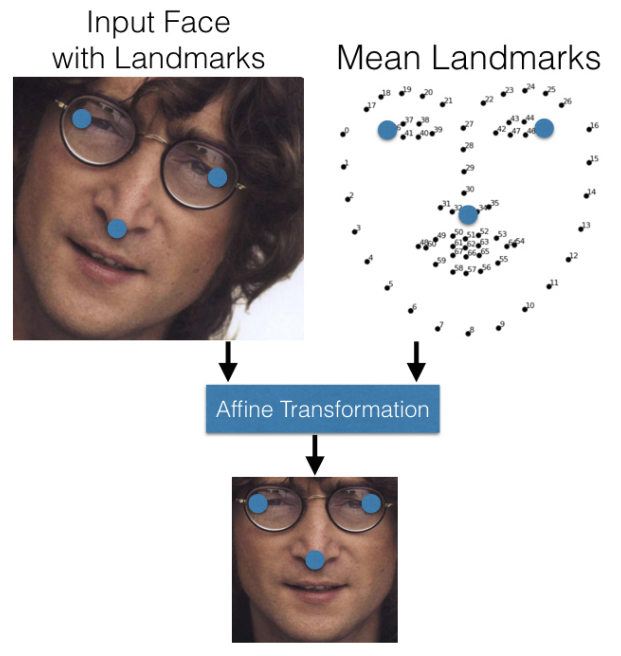
\includegraphics[width=0.5\textwidth]{figures/openface_detection.png}
    \caption{Landmark Detector \cite{amos}}
	\label{fig:meanlandmark}
\end{figure}
}
\end{tabular}  
\end{frame}
\fi

\begin{frame}{Face Detection}
\begin{tabular}{l}
\parbox{1\linewidth}{
\frametitle{Multi-task Cascaded Convolutional Networks (MTCNN)}

%The image is first resized to different scales to build an image pyramid and is the input of the following three stages:

\begin{enumerate}
\item \textbf{Proposal Network (P-Net):} Obtains candidates that will serve as potential positions of the bounding boxes

\item \textbf{Refine Network (R-Net):} Reduce false positives of the first prediction and get the final box boundaries

\item \textbf{Output Network (O-Net):} Outputs landmark positions 

\end{enumerate}
\begin{figure}[!tbp]
 \centering
    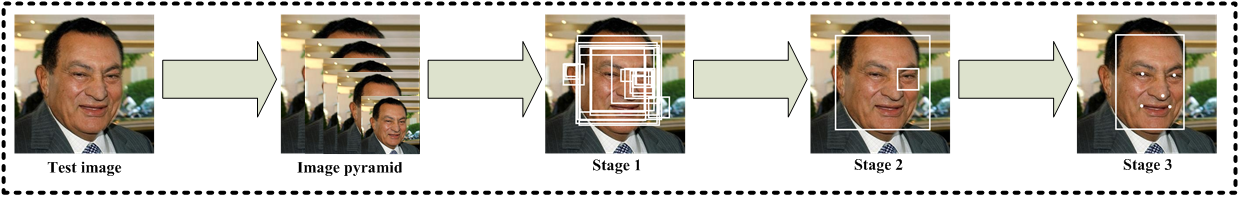
\includegraphics[width=\columnwidth]{figures/mtcnn_pipeline2.png}
    \caption{Cascaded structure with 3 stages of deep CNNs. \cite{zhang}}
	\label{fig:mtcnn}
\end{figure}
}
\end{tabular}  
\end{frame}

\section{Face Representation}
\begin{frame}{Face Representation}
\begin{tabular}{l}
\parbox{1\linewidth}{
\frametitle{Face Representation}
\begin{itemize}
\item The top-performing face representation techniques use CNNs \item Learned robust features of large-scale in-the-wild face datasets directly
\item Optimize the distance between triplets of faces
\item Distances measure the similarity between faces 
\end{itemize}
}
\end{tabular}  
\end{frame}

\begin{frame}{Face Representation}
\begin{tabular}{l}
\parbox{1\linewidth}{
\frametitle{Triplet Loss Function}
\begin{itemize}
\item Separate the distance between two aligned positive face images and an aligned negative face image by a distance margin
\item Result is a feature vector $f(x)$ from a face image $x$ to a compact Euclidean feature space in $ \mathbb{R}^{d}$.
% The distance of the embeddings will be small if the faces are identical and large if the faces are distinct \cite{schroff}.
\end{itemize}
\begin{figure}[!tbp]
 \centering
    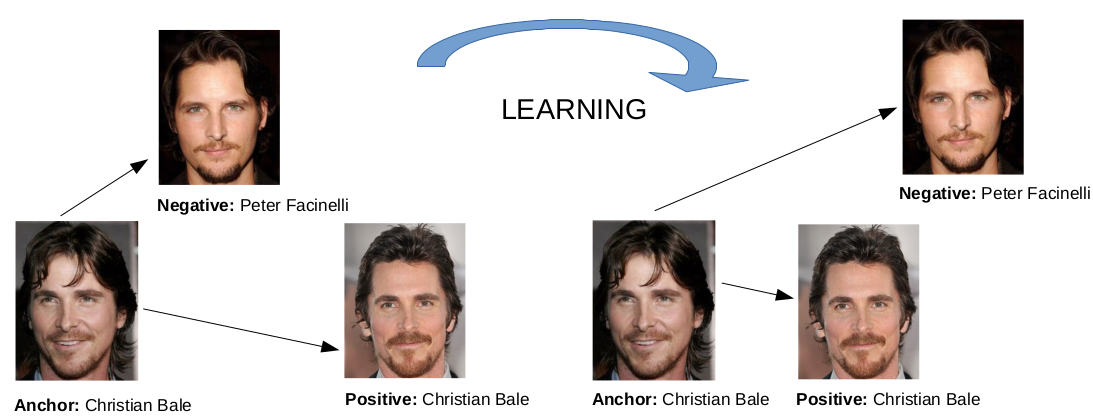
\includegraphics[width=0.8\textwidth]{figures/triplet_loss_example.png}
    \caption{The loss of identical faces are minimized and the loss of distinct faces are maximized \cite{pic1} \cite{pic2}.}
	\label{fig:bale}
\end{figure}
}
\end{tabular}  
\end{frame}

\section{Experiment}
\begin{frame}{Set-Up}
\begin{tabular}{l}
\parbox{1\linewidth}{
\frametitle{Set-Up}
\begin{itemize}
\item Faces of people were clustered by profession
\item \textbf{Feature Extraction Methods: } FaceNet, Dlib, OpenFace, ArcFace 
\item Pre-trained models from each method was used in the experiment
\item \textbf{Clustering algorithms: } K-Means, Spectral, Hierarchical Agglomerative, EM, Birch
\item Number of professions $=$ Number of clusters
\end{itemize}
}
\end{tabular}  
\end{frame}

\begin{frame}{Dataset}
\begin{tabular}{l}
\parbox{1\linewidth}{
\frametitle{Dataset}
\begin{itemize}
\item \textbf{Experiment 1: } $2,180$ unique images of five categories of athletes
\item \textbf{Experiment 2: } $2,065$ unique images of five different categories of professions
\item \textbf{Experiment 3: } $4,593$ unique images of 11 different categories of professions
\item The majority of images from Experiment 2 and 3 are obtained from Wikidata using SPARQL query service
\end{itemize}
}
\end{tabular}  
\end{frame}

\begin{frame}{Dataset}
\begin{tabular}{l}
\parbox{1\linewidth}{
\frametitle{Experiment 1 Dataset}
\begin{figure}[!tbp]
 \centering
    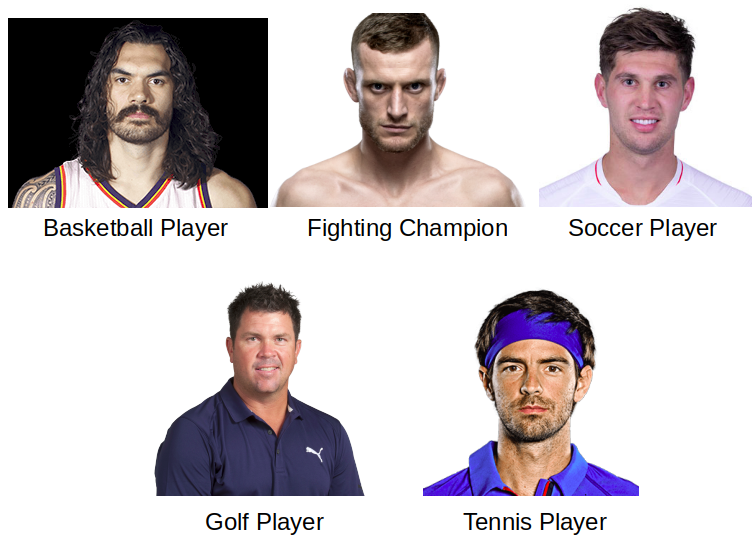
\includegraphics[width=0.8\columnwidth]{figures/ex1.png}
    \caption{Five categories of athletes \cite{data1}}
	\label{fig:sport}
\end{figure}
}
\end{tabular}  
\end{frame}

\begin{frame}{Dataset}
\begin{tabular}{l}
\parbox{1\linewidth}{
\frametitle{Experiment 2 Dataset}
\begin{figure}[!tbp]
 \centering
    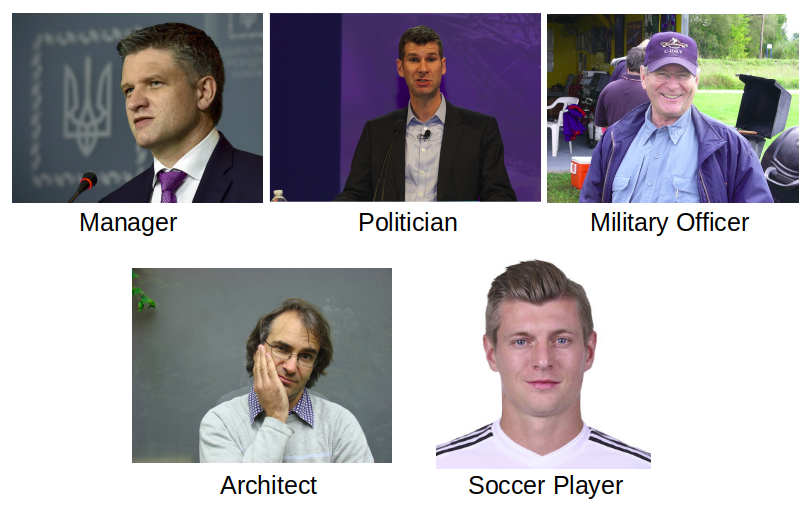
\includegraphics[width=0.8\columnwidth]{figures/ex2.png}
    \caption{Five categories of professions \cite{data1}}
	\label{fig:prof}
\end{figure}
}
\end{tabular}  
\end{frame}

\begin{frame}{Dataset}
\begin{tabular}{l}
\parbox{1\linewidth}{
\frametitle{Experiment 3 Dataset}
\begin{figure}[!tbp]
 \centering
    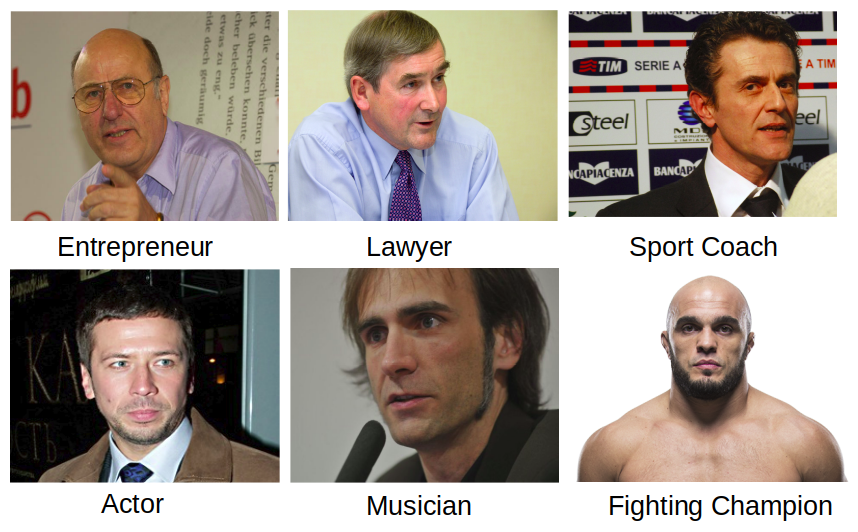
\includegraphics[width=0.8\columnwidth]{figures/ex3.png}
    \caption{In combination with the dataset from Experiment 2: 11 professions}
\end{figure}
}
\end{tabular}  
\end{frame}

\begin{frame}{Feature Extraction Methods}
\begin{tabular}{l}
\parbox{1\linewidth}{
\frametitle{Feature Extraction Methods}

\begin{table}[H]
\centering
\begin{tabular}{||c c c||} 
 \hline
  Method & Face Detector & Number of Features\\ [0.5ex]
 \hline\hline
 \textbf{FaceNet} & MTCNN (160 x 160 px) & 512\\ 
 \hline
 \textbf{Dlib} & HOG & 128\\
 \hline
 \textbf{OpenFace} & HOG (96 x 96 px) & 128\\
 \hline
 \textbf{ArcFace} & MTCNN (112 x 112 px) & 512\\
 \hline
\end{tabular}
\caption{The face detection method used and the number of features of the embeddings extracted from each method \cite{sandberg}, \cite{geitgey}, \cite{amos2016}, \cite{deng2019}.}
\label{table:1}
\end{table}
}
\end{tabular}  
\end{frame}

\begin{frame}{Feature Extraction Methods}
\begin{tabular}{l}
\parbox{1\linewidth}{
\frametitle{Feature Extraction Methods}
\begin{itemize}
\item After face alignment, \textbf{FaceNet, Dlib, OpenFace} use the triplet loss function to learn the embeddings
\item \textbf{ArcFace} uses the additive angular margin which adds a geometric interpretation by rotating the image to a straight face
\end{itemize}

\begin{figure}[!tbp]
 \centering
    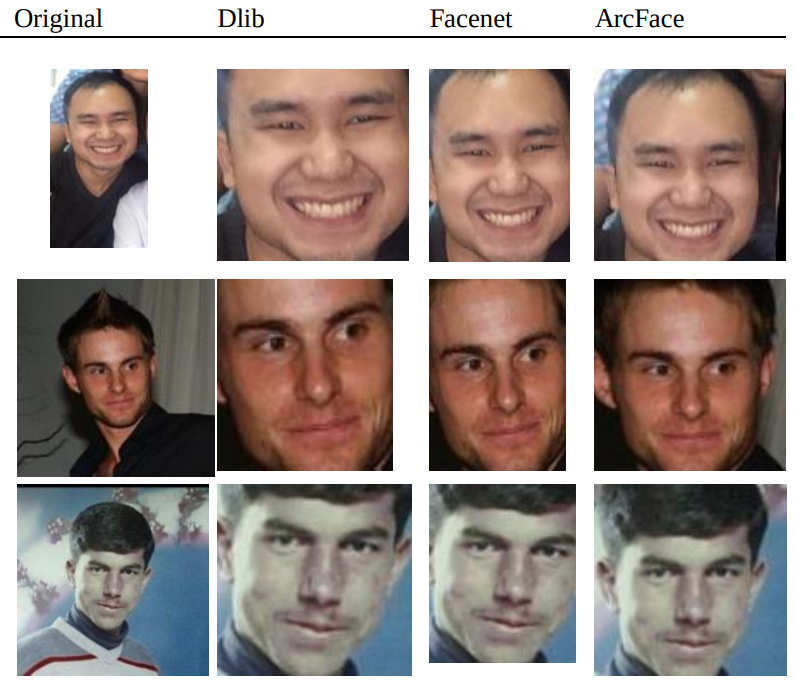
\includegraphics[width=0.5\textwidth]{figures/comparison.png}
	\label{fig:arcface1}
\end{figure}
}
\end{tabular}  
\end{frame}

\begin{frame}{Feature Extraction Methods}
\begin{tabular}{l}
\parbox{1\linewidth}{
\frametitle{Feature Extraction Methods}
\begin{table}[H]
%\centering
\begin{tabular}{||c c c||} 
 \hline
  Method & LFW Accuracy & Training Dataset Size\\ [0.5ex]
 \hline\hline
 \textbf{FaceNet} & 0.9965 & 3.31M images, 9,121 identitie\\ 
 \hline
 \textbf{Dlib} & 0.9938 & 3M images, 7,485 identities\\
 \hline
 \textbf{OpenFace} & 0.9292 & 500k images\\
 \hline
 \textbf{ArcFace} & 0.9982 & 10M images, 100k identities\\
 \hline
 \textbf{Human-Level} \cite{amos} & 0.9753 &\\
 \hline
\end{tabular}
\caption{Accuracy based on the LFW benchmark and training data size of the pre-trained models \cite{sandberg}, \cite{geitgey}, \cite{amos2016}, \cite{deng2019}.}
\label{table:2}
\end{table}

}
\end{tabular}  
\end{frame}

\begin{frame}{Feature Extraction Methods}
\begin{tabular}{l}
\parbox{1\linewidth}{
\frametitle{Feature Extraction Methods}
\begin{table}[H]
\centering
\begin{tabular}{||c c c c||} 
 \hline
  Method & Experiment 1 & Experiment 2 & Experiment 3\\ [0.5ex]
 \hline\hline
 \textbf{FaceNet} & 2,180 x 512 & 2,065 x 512 & 4,593 x 512\\ 
 \hline
 \textbf{Dlib} & 2,180 x 128 & 2,065 x 128 & 4,593 x 128\\
 \hline
 \textbf{OpenFace} & 2,180 x 128 & 2,065 x 128 & 4,593 x 128\\
 \hline
 \textbf{ArcFace} & 2,180 x 512 & 2,065 x 512 & 4,593 x 512\\
 \hline
\end{tabular}
\caption{Dimensions of the feature embeddings extracted from each method}
\label{table:3}
\end{table}
}
\end{tabular}  
\end{frame}

\section{Results}
\begin{frame}{Evaluation}
\begin{tabular}{l}
\parbox{1\linewidth}{
\frametitle{Evaluation: Pairwise F-Measure}
\begin{itemize}
\item Actual Clusters $L = \{\{A1, A2, A3\}, \{B1\}, \{U1, U2\}\}$
\item Cluster Output $C = \{\{A1, A2, B1\}, \{A3, U1, U2 \}\}$
\end{itemize}

\begin{figure}[!tbp]
 \centering
    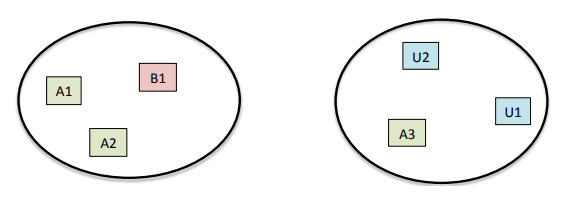
\includegraphics[width=0.8\columnwidth]{figures/fmeasure.png}
    \caption{Example of a possible clustering output. Six data points are grouped into 2 clusters. A1, A2, and A3 have the same label, B1 has it's own label, and U1 and U2 have the same label \cite{otto}.}
    \label{fig:fmeasure}
\end{figure}
}
\end{tabular}  
\end{frame}

\begin{frame}{Evaluation}
\begin{tabular}{l}
\parbox{1\linewidth}{
\frametitle{Evaluation: Pairwise F-Measure}
\begin{itemize}
\item Face pairs from $L$ $P = \{(A1, A2), (A1, A3), (A2, A3), (U1, U2)\}$
\item Face pairs from $C$ \\$Q = \{(A1, A2), (A1, B1), (A2, B1), (A3, U1), (A3, U2), (U1, U2)\}$
\end{itemize}

\begin{figure}[!tbp]
 \centering
    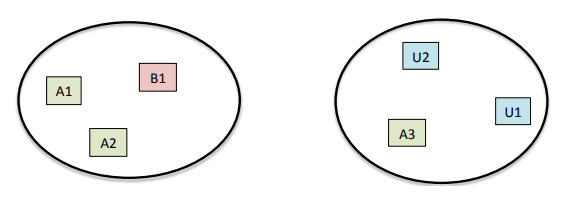
\includegraphics[width=0.8\columnwidth]{figures/fmeasure.png}
    \label{fig:fmeasure}
\end{figure}
}
\end{tabular}  
\end{frame}

\begin{frame}{Evaluation}
\begin{tabular}{l}
\parbox{1\linewidth}{
\frametitle{Evaluation: Pairwise F-Measure}
\begin{itemize}
\item \textbf{True Positives (TP):} The number of face pairs $(i, j)$ that are correctly clustered into the same cluster.

$$TP = | P \cap Q | = |\{(A1, A2), (U1, U2)\}| = 2$$

\end{itemize}

\begin{figure}[!tbp]
 \centering
    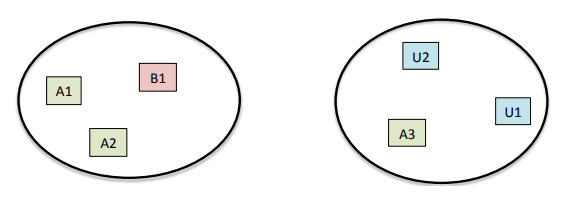
\includegraphics[width=0.8\columnwidth]{figures/fmeasure.png}
    \label{fig:fmeasure}
\end{figure}
}
\end{tabular}  
\end{frame}

\begin{frame}{Evaluation}
\begin{tabular}{l}
\parbox{1\linewidth}{
\frametitle{Evaluation: Pairwise F-Measure}
\begin{itemize}
\item \textbf{False Positives (FP):} The number of face pairs $(i, j)$ that are incorrectly clustered to the same cluster.

$$FP = |Q - P| = |\{(A1, B1), (A2, B1), (A3, U1), (A3, U2)\}| = 4$$ 

\end{itemize}

\begin{figure}[!tbp]
 \centering
    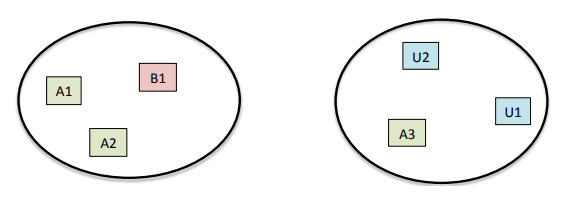
\includegraphics[width=0.8\columnwidth]{figures/fmeasure.png}
    \label{fig:fmeasure}
\end{figure}
}
\end{tabular}  
\end{frame}

\begin{frame}{Evaluation}
\begin{tabular}{l}
\parbox{1\linewidth}{
\frametitle{Evaluation: Pairwise F-Measure}
\begin{itemize}
\item \textbf{False Negatives (FN)}: The number of face pairs that are clustered to a different cluster.

$$FN = |P - Q| = |\{(A1, A3), (A2, A3)\}| = 2$$

\end{itemize}

\begin{figure}[!tbp]
 \centering
    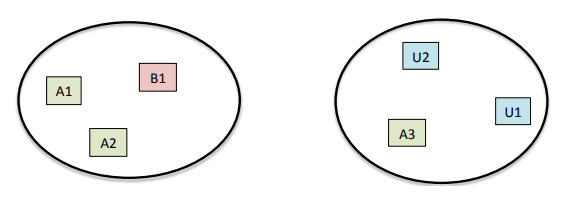
\includegraphics[width=0.8\columnwidth]{figures/fmeasure.png}
    \label{fig:fmeasure}
\end{figure}
}
\end{tabular}  
\end{frame}

\begin{frame}{Evaluation}
\begin{tabular}{l}
\parbox{1\linewidth}{
\frametitle{Evaluation: Pairwise F-Measure}

$$ Pairwise \ Precision = \frac{TP}{TP + FP}$$
\\
$$ Pairwise \ Recall = \frac{TP}{TP + FN}$$
\\
$$Pairwise \ F\textrm{-}Measure = \frac{2 * \textrm{Precision}*\textrm{Recall}}{\textrm{Precision} + \textrm{Recall}}$$

}
\end{tabular}  
\end{frame}

\begin{frame}{Results}
\begin{tabular}{l}
\parbox{1\linewidth}{
\frametitle{Experiment 1 Results}

\begin{table}[H]
\centering
\begin{tabular}{||c c c c c||}
 \hline
Method & FaceNet & Dlib & OpenFace & ArcFace\\ [0.5ex]
 \hline\hline
 \textbf{K-Means} & 0.478 & 0.391 & 0.382 & \textbf{0.516}\\ 
 \hline
  \textbf{Spectral} & 0.445 & 0.361 & 0.345 & \textbf{0.467}\\
 \hline
 \textbf{HAC} & \textbf{0.447} & 0.362 & 0.391 & 0.413\\
 \hline
 \textbf{EM} & 0.449 & 0.394 & 0.376 & \textbf{0.512}\\
 \hline
 \textbf{Birch} & 0.442 & 0.404 & 0.331 & \textbf{0.453}\\
 \hline
\end{tabular}
\caption{F-Measure obtained by each feature extraction and clustering method}
\label{table:ex1}
\end{table}

}
\end{tabular}  
\end{frame}

\begin{frame}{Results}
\begin{tabular}{l}
\parbox{1\linewidth}{
\frametitle{Experiment 1 True Positives}

\begin{figure}[H]
 \centering
    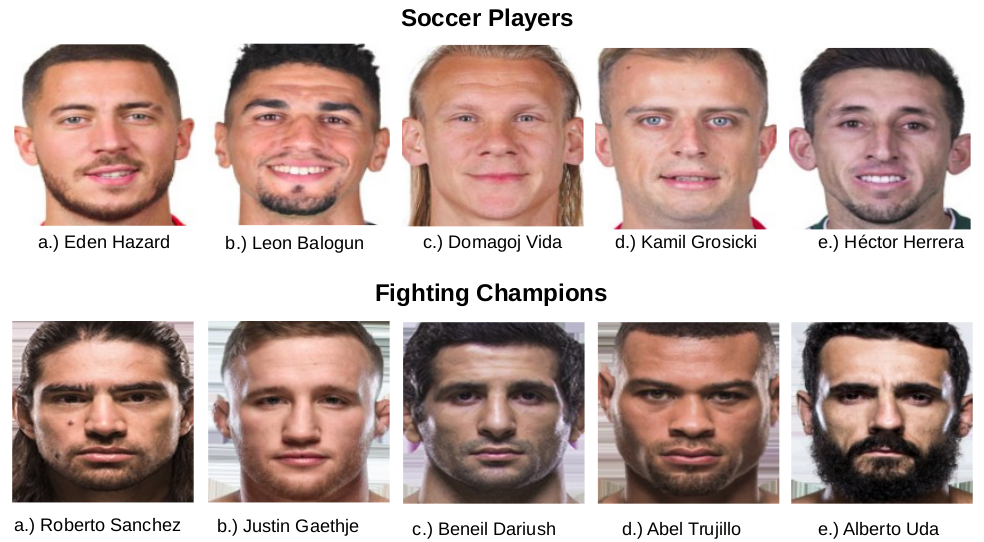
\includegraphics[width=0.9\columnwidth]{figures/soccer_tp.png}
    \caption{\textbf{True Positives} using FaceNet and K-Means. Clusters of Soccer Players and Fighting Champions.}
    \label{fig:ex1tp}
\end{figure}

}
\end{tabular}  
\end{frame}

\begin{frame}{Results}
\begin{tabular}{l}
\parbox{1\linewidth}{
\frametitle{Experiment 1 False Positives and False Negatives}

\begin{figure}[H]
  \centering
  \begin{minipage}[b]{0.4\textwidth}
    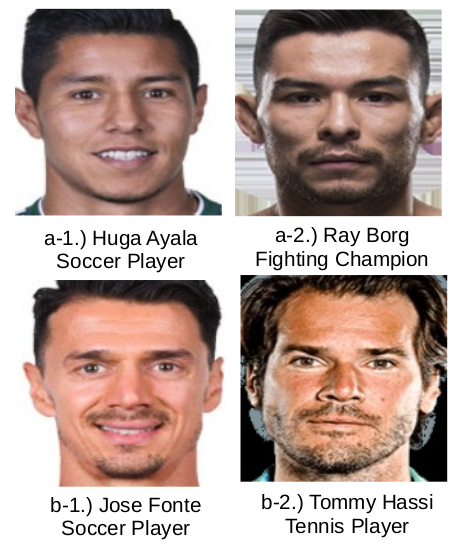
\includegraphics[width=\textwidth]{figures/soccer_fp.png}
    \caption{\textbf{False Positives}}
    \label{fig:ex1fp}
  \end{minipage}
  \hfill
  \begin{minipage}[b]{0.4\textwidth}
    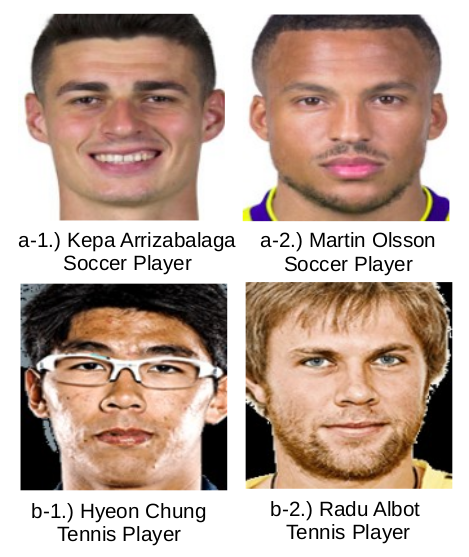
\includegraphics[width=\textwidth]{figures/soccer_fn.png}
    \caption{\textbf{False Negatives}}
    \label{fig:ex1fn}
  \end{minipage}
\end{figure}

}
\end{tabular}  
\end{frame}

\begin{frame}{Results}
\begin{tabular}{l}
\parbox{1\linewidth}{
\frametitle{Experiment 2 Results}
\begin{table}[H]
\centering
\begin{tabular}{||c c c c c||} 
 \hline
Method & FaceNet & Dlib & OpenFace & ArcFace\\ [0.5ex]
 \hline\hline
 \textbf{K-Means} & \textbf{0.426} & 0.405 & 0.306 & 0.294\\ 
 \hline
  \textbf{Spectral} & \textbf{0.392} & 0.367 & 0.295 & 0.272\\
 \hline
 \textbf{HAC} & 0.384 & \textbf{0.392} & 0.310 & 0.333\\
 \hline
 \textbf{EM} & \textbf{0.443} & 0.411 & 0.310 & 0.277\\
 \hline
 \textbf{Birch} & \textbf{0.399} & 0.383 & 0.294 & 0.304\\
 \hline
\end{tabular}
\caption{Experiment 2 F-Measure Comparison}
\label{table:ex2}
\end{table}

}
\end{tabular}  
\end{frame}

\begin{frame}{Results}
\begin{tabular}{l}
\parbox{1\linewidth}{
\frametitle{Experiment 2 True Positives}
\begin{figure}[H]
 \centering
    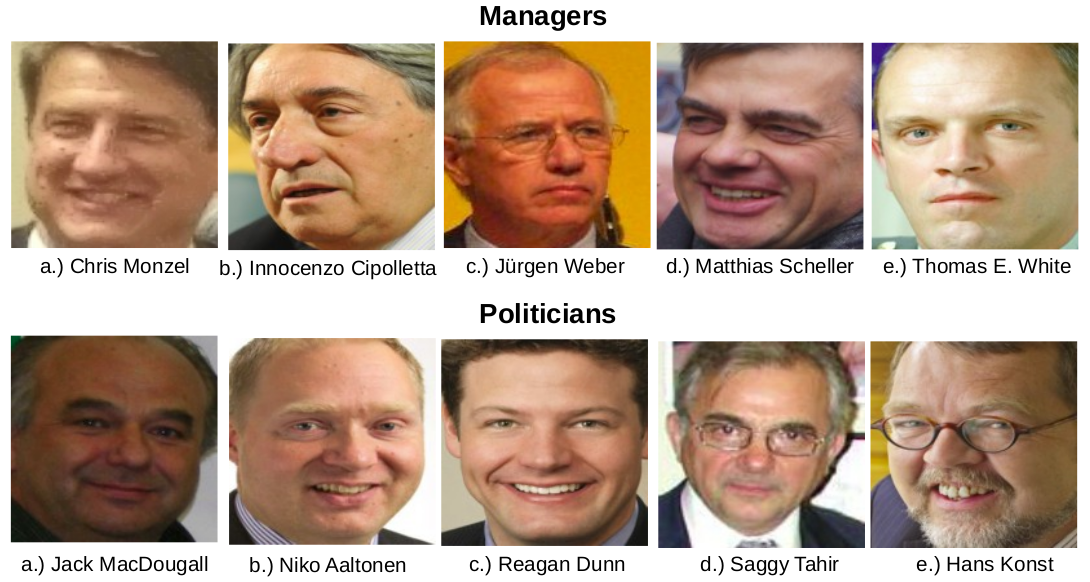
\includegraphics[width=\columnwidth]{figures/manager.png}
    \caption{Experiment 2: \textbf{True Positives} using FaceNet and K-Means. Cluster of Managers and Politicians}
    \label{fig:ex2tp}
\end{figure}

}
\end{tabular}  
\end{frame}

\begin{frame}{Results}
\begin{tabular}{l}
\parbox{1\linewidth}{
\frametitle{Experiment 3 Results}
\begin{table}[H]
\centering
\begin{tabular}{||c c c c c||} 
 \hline
Method & FaceNet & Dlib & OpenFace & ArcFace\\ [0.5ex]
 \hline\hline
 \textbf{K-Means} & \textbf{0.203} & 0.185 & 0.141 & 0.182\\ 
 \hline
  \textbf{Spectral} & \textbf{0.204} & 0.166 & 0.143 & 0.159\\
 \hline
 \textbf{HAC} & 0.177 & \textbf{0.188} & 0.131 & 0.174\\
 \hline
 \textbf{EM} & \textbf{0.210} & 0.191 & 0.146 & 0.179\\
 \hline
 \textbf{Birch} & 0.182 & \textbf{0.193} & 0.149 & 0.151\\
 \hline
\end{tabular}
\caption{Experiment 3 F-Measure Comparison}
\label{table:ex3}
\end{table}
}
\end{tabular}  
\end{frame}

\begin{frame}{Results}
\begin{tabular}{l}
\parbox{1\linewidth}{
\frametitle{Experiment 3 True Positives}
\begin{figure}[H]
 \centering
    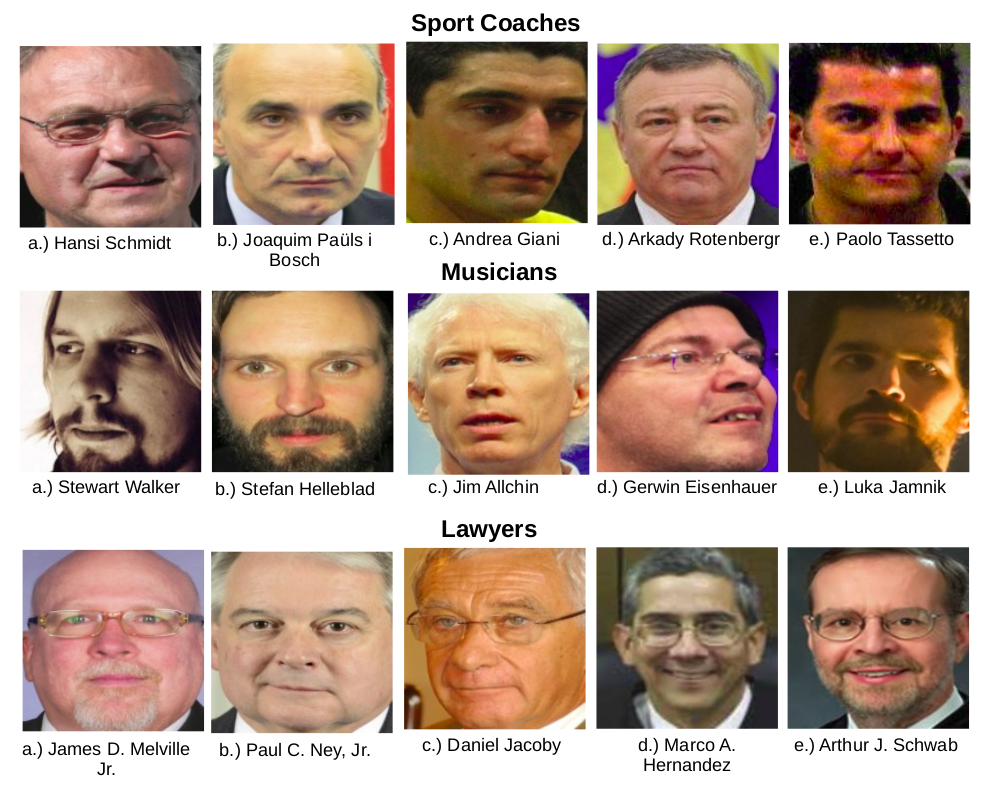
\includegraphics[width=0.5\columnwidth]{figures/lawyers.png}
    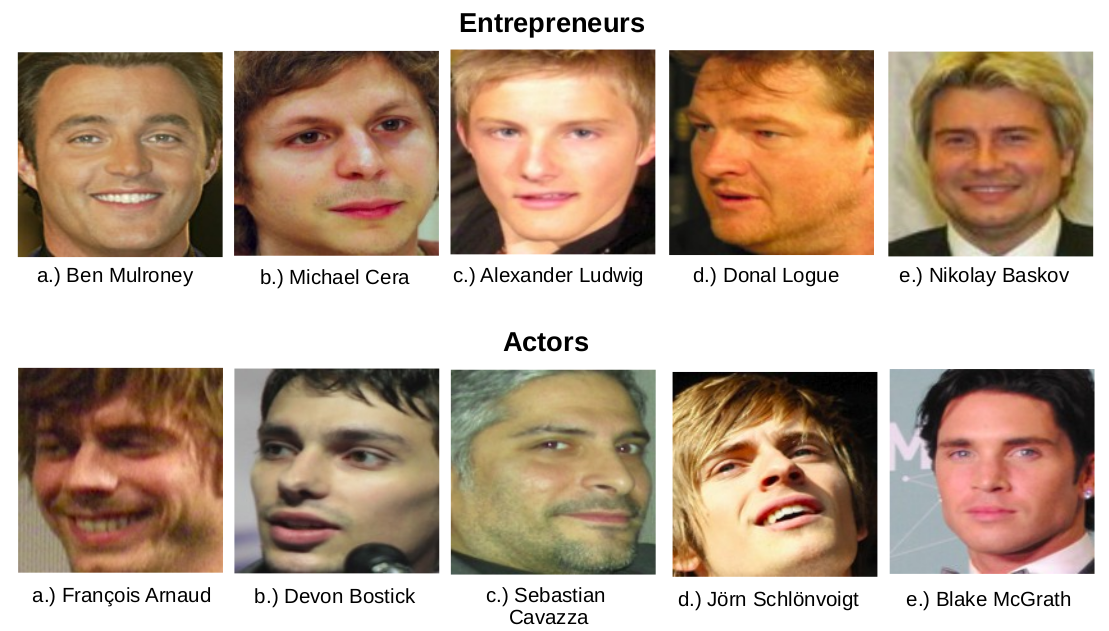
\includegraphics[width=0.5\columnwidth]{figures/actor.png}
    \caption{Experiment 3: \textbf{True Positives} using FaceNet and K-Means. Cluster of Sport Coaches, Musicians, Lawyers, Entrepreneurs, and Actors}
    \label{fig:ex2tp}
\end{figure}

}
\end{tabular}  
\end{frame}

\begin{frame}{Results}
\begin{tabular}{l}
\parbox{1\linewidth}{
\frametitle{Experiment 3 False Positives and False Negatives}
\begin{figure}[H]
  \centering
  \begin{minipage}[b]{0.4\textwidth}
    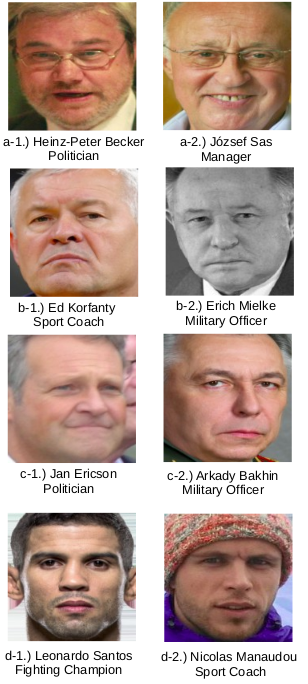
\includegraphics[width=\textwidth]{figures/ex2_fp.png}
    \caption{\textbf{False Positives}}
    \label{fig:ex2fp}
  \end{minipage}
  \hfill
  \begin{minipage}[b]{0.4\textwidth}
   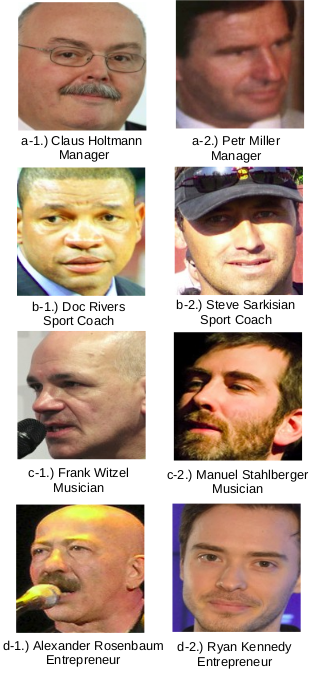
\includegraphics[width=\textwidth]{figures/ex2_fn.png}
    \caption{\textbf{False Negatives}}
    \label{fig:ex2fn}
  \end{minipage}
\end{figure}

}
\end{tabular}  
\end{frame}

\begin{frame}{Results}
\begin{tabular}{l}
\parbox{1\linewidth}{
\frametitle{Analysis}
\begin{itemize}
\item Experiment 1: The highest F-Measure was 0.516 using \textbf{ArcFace and K-Means clustering}
\item Experiment 2: The highest F-Measure was 0.443 using \textbf{FaceNet and EM clustering}
\item Experiment 3: The highest F-Measure was 0.210 using \textbf{FaceNet and EM clustering}
\end{itemize}

}
\end{tabular}  
\end{frame}

\begin{frame}{Results}
\begin{tabular}{l}
\parbox{1\linewidth}{
\frametitle{Analysis}
\begin{table}[h!]
\centering
\begin{tabular}{||c c c c||} 
 \hline
Method & Experiment 1 & Experiment 2 & Experiment 3\\ [0.5ex]
 \hline\hline
 \textbf{FaceNet} & \textbf{00:15:06} & \textbf{00:25:27} & 00:57:44\\ 
 \hline
  \textbf{Dlib} & 00:28:19 & 00:50:44 & 01:52:57\\
 \hline
 \textbf{OpenFace} & 00:16:01 & 00:27:59 & \textbf{00:53:30}\\
 \hline
 \textbf{ArcFace} & 00:16:04 & 00:42:44 & 01:34:38\\
 \hline
\end{tabular}
\caption{Runtime to align and extract faces}
\label{table:runtime}
\end{table}

}
\end{tabular}  
\end{frame}

\section{Conclusion}

\begin{frame}{Results}
\begin{tabular}{l}
\parbox{1\linewidth}{
\frametitle{Conclusion}
\begin{itemize}
\item ArcFace is a good choice for images with high-quality head \item FaceNet is a better choice in terms of consistency, accuracy, and efficiency for in-the-wild images
\item K-Means and EM Clustering provided the highest accuracy for the experiments
\item Experiments 1 and 2 show a positive correlation between facial features and the person's professional domain
\end{itemize}

}
\end{tabular}  
\end{frame}



\printbibliography


\end{document}
